% ============================================================
%  Experiment 5 --- Interfacing FPGA to Analog-to-Digital Converter
%  (renumbered from the former Experiment 9)
% ============================================================
\experimentheader{5}{Experiment 5}{Interfacing FPGA to Analog-to-Digital Converter}{FPGA Lab}

\begin{objectives}
  \begin{enumerate}
    \item To understand the operation of an analog-to-digital converter (ADC).
    \item To interface an FPGA, via the Altera DE2 board, to an ADC.
  \end{enumerate}
\end{objectives}

\begin{equipment}
  \begin{enumerate}
    \item Altera Quartus II software
          \begin{itemize}
            \item version 9/10/12 for Cyclone II
            \item version 9/10/12/latest for Cyclone IV
          \end{itemize}
    \item Altera DE2 board
    \item Multimeter / oscilloscope
    \item ADC0804 analog-to-digital converter
    \item Resistors: $10\,\text{k}\Omega$
    \item Variable resistor (potentiometer), $10\,\text{k}\Omega$
    \item Capacitor: $150\,\text{pF}$
    \item 8 LEDs
    \item 74LS245 octal bus transceiver
  \end{enumerate}
\end{equipment}

\begin{introduction}
  This experiment explores interfacing an ADC chip to an FPGA. ADCs are among the most widely used data-acquisition devices: they translate an analog signal into a digital number that a processor (or, here, an FPGA) can read. A widely used ADC is the ADC0804 (National Semiconductor): it operates from $+5\,\text{V}$ and has 8-bit resolution.\vspace*{0.5em}

  Besides resolution, \textit{conversion time} is a major factor in judging an ADC: the time the ADC takes to convert its analog input to a digital number. For the ADC0804 this depends on the clock signal applied to the CLK\,R / CLK\,IN pins, but cannot be faster than $110\,\mu\text{s}$.\vspace*{0.5em}

  The ADC0804's input range is set by the $V_{ref}/2$ pin, as shown in Table~\ref{tab:exp9-vref}. The chip's outputs are 5\,V logic; since the DE2 board's inputs only tolerate 3.3\,V, an octal bus transceiver (74LS245) must be used to step the output voltage down before it reaches the FPGA.

  \begin{center}
    \[
      D_{out} = \frac{V_{in}}{\text{step size}}
    \]
  \end{center}
  where $D_{out}$ is the digital data output and $V_{in}$ is the analog input voltage.

  Data conversion with the ADC0804 follows this sequence (Figure~\ref{fig:exp9-timing}):
  \begin{enumerate}[label=\roman*.]
    \item Set $\overline{\text{CS}} = 0$ and send a low-to-high pulse on the $\overline{\text{WR}}$ pin to start the conversion.
    \item Monitor the $\overline{\text{INTR}}$ pin: while it is high, the conversion is still in progress; once it goes low, the conversion is complete.
    \item With $\overline{\text{INTR}}$ low, set $\overline{\text{CS}} = 0$ again and send a high-to-low pulse on the $\overline{\text{RD}}$ pin to read the data out of the ADC0804.
  \end{enumerate}
\end{introduction}

\needspace{4cm}
\begin{boxedtable}
  \captionof{table}{$V_{ref}/2$ relation to $V_{in}$ range.}
  \label{tab:exp9-vref}
  {\renewcommand{\arraystretch}{1.5}
    \centering
    \begin{tabular}{lll}
      \toprule
      $V_{ref}/2$ (V) & $V_{in}$ range (V) & Step size (mV)     \\
      \midrule
      Not connected   & 0 to 5             & $5/256 = 19.53$    \\
      2.0             & 0 to 4             & $4/255 = 15.62$    \\
      1.5             & 0 to 3             & $3/256 = 11.71$    \\
      1.28            & 0 to 2.56          & $2.56/256 = 10.00$ \\
      1.0             & 0 to 2             & $2/256 = 7.81$     \\
      0.5             & 0 to 1             & $1/256 = 3.90$     \\
      \bottomrule
    \end{tabular}
  }
\end{boxedtable}

\begin{boxedfigure}
  \centering
  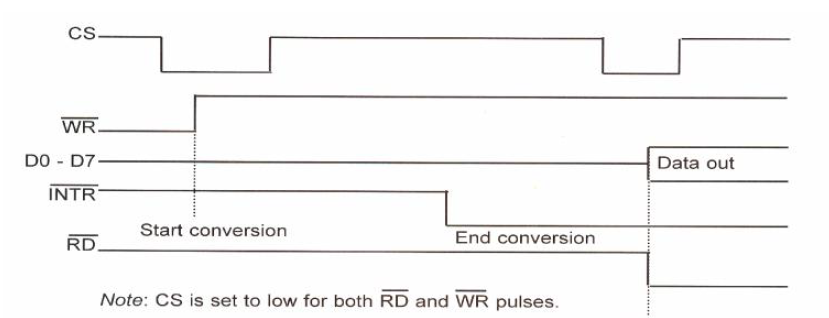
\includegraphics[width=0.85\linewidth]{figures/Exp9_Figure_1.png}

  \vspace{4pt}
  \captionof{figure}{Read and write timing for the ADC0804.}
  \label{fig:exp9-timing}
\end{boxedfigure}

\begin{procedure}

  \textbf{Activity 1 --- Free-running mode}\vspace{2pt}

  \textit{Objective: run the ADC0804 in free-running mode.}

  \begin{enumerate}
    \item Connect the ADC0804 as shown in Figure~\ref{fig:exp9-circuit} for free-running mode.
    \item Vary the input signal from 0 to 5\,V using the $10\,\text{k}\Omega$ potentiometer shown in Figure~\ref{fig:exp9-circuit} as the ADC's input. The input must not exceed 5\,V.
    \item Tabulate your results in Table~\ref{tab:exp9-freerun}.
    \item Compare your hardware result with the value calculated using Equation~(1).
  \end{enumerate}

  \begin{boxedfigure}
    \centering
    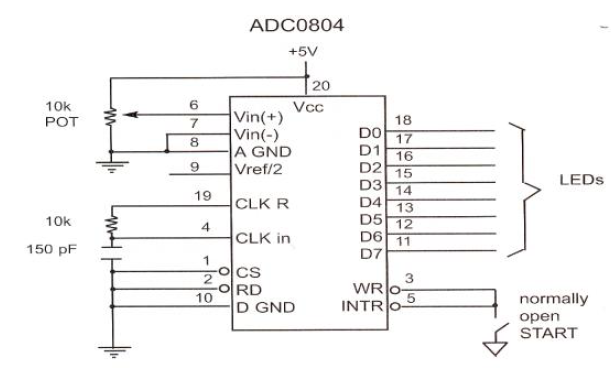
\includegraphics[width=0.75\linewidth]{figures/Exp9_Figure_2.png}
    \captionof{figure}{ADC0804 test circuit for free-running mode.}
    \label{fig:exp9-circuit}
  \end{boxedfigure}

  \needspace{4cm}
  \begin{boxedtable}
    \captionof{table}{Free-running mode output.}
    \label{tab:exp9-freerun}
    {\renewcommand{\arraystretch}{1.5}
      \centering
      \begin{tabular}{cccc}
        \toprule
        \# & Input (V) & Output (hardware) & Output (calculation) \\
        \midrule
        1  & 0.0       &                   &                      \\
        2  & 0.5       &                   &                      \\
        3  & 1.0       &                   &                      \\
        4  & 1.5       &                   &                      \\
        5  & 2.0       &                   &                      \\
        6  & 2.5       &                   &                      \\
        7  & 3.0       &                   &                      \\
        8  & 3.5       &                   &                      \\
        9  & 4.0       &                   &                      \\
        10 & 4.5       &                   &                      \\
        \bottomrule
      \end{tabular}
    }
  \end{boxedtable}
  \vspace*{1.5em}

  \textbf{Activity 2 --- Interfacing the ADC to the FPGA, displaying on LEDs}\vspace{2pt}

  \textit{Objective: interface the ADC to the FPGA and display the digitised result on LEDs.}

  \begin{enumerate}
    \item Use the circuit from Figure~\ref{fig:exp9-circuit}, modified as follows.
    \item Connect the $\overline{\text{RD}}$ and $\overline{\text{WR}}$ pins to general-purpose I/O pins on the DE2 board, declared as \textbf{outputs}.
    \item Connect the $\overline{\text{INTR}}$ and D0--D7 pins to the inputs of a 74LS245. Connect the 74LS245's outputs to general-purpose I/O pins on the DE2 board, declared as \textbf{inputs}. Refer to the DE2 user manual for pin locations.
    \item In Verilog, generate the $\overline{\text{WR}}$ pulse to start conversion, poll $\overline{\text{INTR}}$ for end of conversion, then pulse $\overline{\text{RD}}$ to read the data on D0--D7.
    \item Assign the FPGA's digitised outputs to the LED pins.
    \item Compile, simulate, and download the program to the DE2 board.
    \item Use the potentiometer to vary the input value.
    \item Tabulate your results in Table~\ref{tab:exp9-fpga}.
    \item Print and submit the Verilog code, simulation result, and experimental results.
  \end{enumerate}

  \needspace{4cm}
  \begin{boxedtable}
    \captionof{table}{FPGA-interfaced ADC output.}
    \label{tab:exp9-fpga}
    {\renewcommand{\arraystretch}{1.5}
      \centering
      \begin{tabular}{cc c}
        \toprule
        \# & Input (V) & Output \\
        \midrule
        1  & 0.8       &        \\
        2  & 1.7       &        \\
        3  & 2.3       &        \\
        4  & 2.8       &        \\
        5  & 3.1       &        \\
        6  & 3.6       &        \\
        7  & 3.9       &        \\
        8  & 4.1       &        \\
        9  & 4.6       &        \\
        10 & 4.8       &        \\
        \bottomrule
      \end{tabular}
    }
  \end{boxedtable}
  \vspace*{1.5em}

  \textbf{Activity 3 --- Displaying the ADC result on the LCD}\vspace{2pt}

  \textit{Objective: interface the ADC0804 to the DE2 board and display the result on the LCD.}

  \begin{enumerate}
    \item Using the same circuit as in Activity 2, write Verilog code to read data from the ADC and display the result on the LCD (see Experiment 5 for the LCD interface).
    \item Print and submit the Verilog code and simulation result.
  \end{enumerate}

\end{procedure}
